\documentclass{beamer}
\usepackage[latin1]{inputenc}
\usetheme{Warsaw}
\title[Make a LaTeX presentation using Beamer]{Introduction  to Beamer\\How to make a presentation with LaTeX?}
\author{Nadir Soualem -- Astozzia}
\institute{Math-linux.com}
\date{Jule 13, 2007}
\begin{document}

\begin{frame}
\begin{figure}
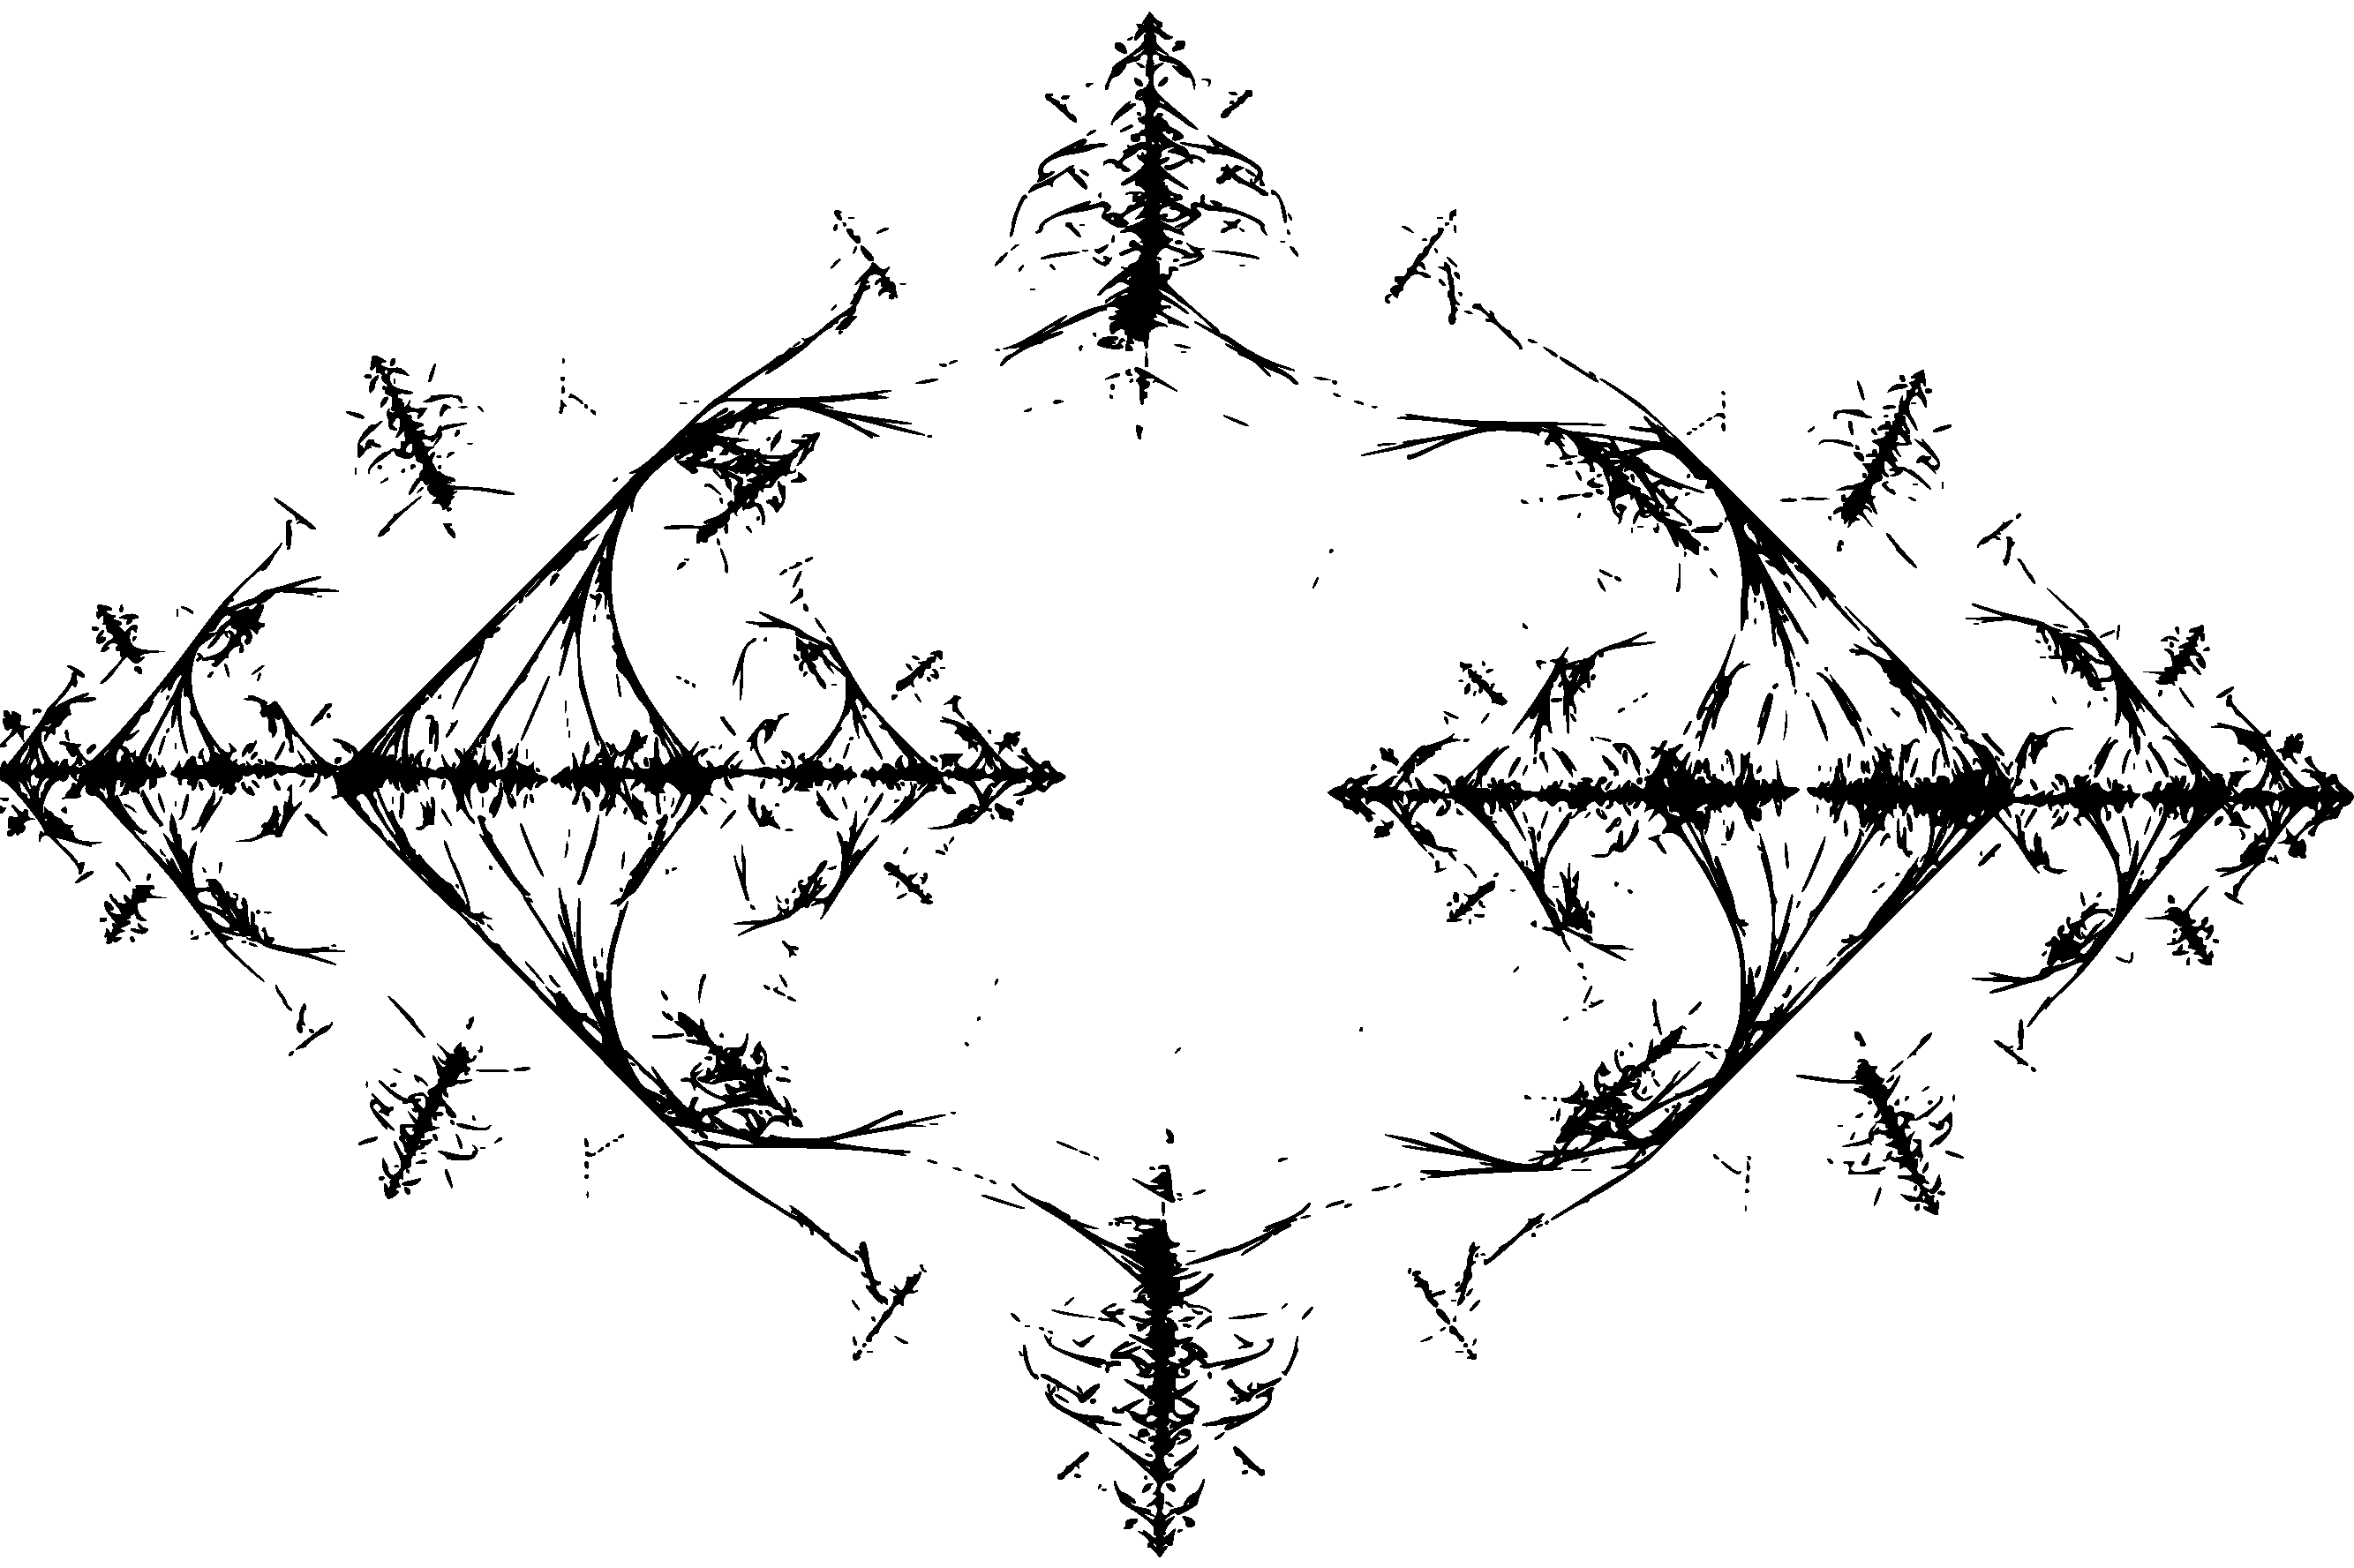
\includegraphics[scale=0.2]{test2}
\end{figure}

\end{frame}

\begin{frame}

\begin{itemize}
\item Language used by Beamer: L\uncover<2->{A}TEX
\item Language used by Beamer: L\only<2->{A}TEX
\end{itemize}

\begin{block}{Block title}
This is a block in blue
\end{block}

\begin{alertblock}{Alert-block title}
This is a block in red
\end{alertblock}

\begin{exampleblock}{Example-block title}
This is a block in green
\end{exampleblock}
\end{frame}

\begin{frame}
\begin{itemize}[<+->]
\item L
\item A
\item T
\item E
\item X
\end{itemize}
\end{frame}

\begin{frame}
\begin{itemize}
\item Beamer is a wonderful class
\pause \item One can make animations
\pause \item One uses the\textbf{pause} command, for example
\pause \item in order to bring in important ideas
\end{itemize}
\end{frame}
\end{document}
